\documentclass{article}
\usepackage[utf8]{inputenc}
\usepackage{amsmath}
\usepackage{systeme}
\usepackage[most]{tcolorbox}
\usepackage[scale=.95,type1]{cabin}
\usepackage{lmodern}

\usepackage[legalpaper,margin=1in]{geometry}

\setlength{\parindent}{10pt}
\setlength{\parskip}{1em}
\renewcommand{\baselinestretch}{1.2}

\title{Matrices}
\date{}

\newcounter{example}[section]
\newenvironment{example}[1][]{\refstepcounter{example}\par\medskip
   \noindent \textbf{Example~\theexample. #1} \rmfamily}{\medskip}

\makeatletter
\renewcommand*\env@matrix[1][*\c@MaxMatrixCols c]{%
  \hskip -\arraycolsep
  \let\@ifnextchar\new@ifnextchar
  \array{#1}}
\makeatother

\newcommand\y{\cellcolor{blue!10}}
\newcommand\B{\textbf}
\newcommand\tcl{\begin{tcolorbox}[colback = {blue9}]}
\newcommand\etcl{\end{tcolorbox}}

\usepackage{tabularray}
\SetTblrInner{colsep=5pt,rowsep=1pt}

\newcommand\x{\times}

\makeatletter
\newcommand{\dashover}[2][\mathop]{#1{\mathpalette\df@over{{\dashfill}{#2}}}}
\newcommand{\fillover}[2][\mathop]{#1{\mathpalette\df@over{{\solidfill}{#2}}}}
\newcommand{\df@over}[2]{\df@@over#1#2}
\newcommand\df@@over[3]{%
  \vbox{
    \offinterlineskip
    \ialign{##\cr
      #2{#1}\cr
      \noalign{\kern1pt}
      $\m@th#1#3$\cr
    }
  }%
}
\newcommand{\dashfill}[1]{%
  \kern-.5pt
  \xleaders\hbox{\kern.5pt\vrule height.4pt width \dash@width{#1}\kern.5pt}\hfill
  \kern-.5pt
}
\newcommand{\dash@width}[1]{%
  \ifx#1\displaystyle
    2pt
  \else
    \ifx#1\textstyle
      1.5pt
    \else
      \ifx#1\scriptstyle
        1.25pt
      \else
        \ifx#1\scriptscriptstyle
          1pt
        \fi
      \fi
    \fi
  \fi
}
\newcommand{\solidfill}[1]{\leaders\hrule\hfill}
\makeatother

\begin{document}
    
    \section{Determinant of a matrix}
        Historically, the use of determinants arose from the recognition of \textbf{special patterns} that occur
        in the \textbf{solutions} of systems of linear equations. For instance, the general solution of the system 
        \begin{equation*}
            \begin{matrix}
                a_{11}x_1 + a_{12}x_2 = b_1 \\
                a_{21}x_1 + a_{22}x_2 = b_2
            \end{matrix}
        \end{equation*}
        can be shown to be 
        \begin{center}
            $x_1 = \frac{b_1a_{22} - b_2a_{12}}{a_{11}a_{22} - a_{21}a_{12}}$ and $x_2 = \frac{b_2a_{11} - b_1a_{21}}{a_{11}a_{22} - a_{21}a_{12}} $,
        \end{center}
        provided that $a_{11}a_{22} - a_{21}a_{12} \neq 0$. Note that both fractions have the same \B{denominator}. This quantity
        is called the determinant of the coefficient matrix $A$.

        \begin{tcolorbox}[colback = {blue9}]
            The \B{determinant} of the matrix 
            \[ A = \begin{bmatrix}
                a_{11} & a_{12} \\
                a_{21} & a_{22}
            \end{bmatrix}\]
            is given by
            \[ det(A) = |A| = a_{11}a_{22} - a_{21}a_{21}\]
        \end{tcolorbox}

        \subsubsection*{\textcolor{blue}{For matrix of order higher than $2$}}
            
        \tcl
        The \B{minor} $M_{ij}$ of the element $a_{ij}$ is the \textit{determinant} of the matrix obtained by \textit{deleting} the $i$th row
        and the $j$th column. The \B{cofactor} $C_{ij}$ is given by 
        \[C_{ij} = (-1)^{i+j}M_{ij}\]
        \etcl
        To obtain the cofactors of a matrix, first find the minors then apply the sign $+$ or $-$.

        \subsection*{\textcolor{blue}{DETERMINANT OF A MATRIX}}
        The next definition is called \B{inductive} since it uses determinants of matrices of order $n - 1$ to 
        define the determinant of a matrix of order $n$.
        \subsubsection*{Laplace's Expansion of a Determinant - \textit{expansion by Cofactors}}
        \tcl
            $|A|$ is the sum of the entries in \B{any row or column} of $A$ multiplied by their cofactors
            \[det(A) = |A| = \sum_{j=1}^n a_{1j}C_{1j} = a_{11}C_{11} + a_{12}C_{12} + \dots + a_{n1}C_{n1}\]
            \begin{center}
                \footnotesize \textit{(expanding by cofactors in the first row)}
            \end{center}
            \[|A| = \sum_{i = 1}^n a_{1i}C_{1i} = a_{11}C_{11} + a_{12}C_{12} + \dots + a_{1n}C_{1n}\]
            \begin{center}
                \footnotesize \textit{(expanding by cofactors in the first column)}
            \end{center}
        \etcl
        The row or column that containing the most zeros is usually the best choice for expansion by cofactors.
        
        \subsubsection*{Determinant of a $3 \x 3$ matrix}

        \begin{center}
            \includegraphics*[width = 5cm]{images/det3.png}
        \end{center}

        \subsection*{\textcolor{blue}{Triangular Matrices}}

    \begin{equation*}\label{eq:appendrow}
            \left[\begin{tblr}{
            colspec = {cccc},
            cell{1}{1} = {blue9},
            cell{2}{1,2} = {blue9},
            cell{3}{1,2,3} = {blue9}}
            1 & 2 & -1 & 4 \\
            0 & 1 & 0 & 3 \\
            0 & 0 & 1 & -2
             \end{tblr}\right]
        \end{equation*}

        \tcl
        Determinant of a triangular matrix is the product of its entries on the main diangonal 
        \[det(A) = |A| = a_{11}a_{22}\dots a_{nn} \]
        \etcl

        \subsection{The Effects of Elementary Row Operations on a Determinant}
        \tcl
        \begin{enumerate}
            \item Interchanging 2 rows of $A$, then
                \[det(B) = -det(A)\]
            \item Adding a multiple of a row to \B{another row}
                \[det(B) = det(A)\]
            \item Multiplying a row with $c \neq 0$
                \[det(B) = c.det(A)\]
        \end{enumerate}
        \etcl

        To prove \B{Property 1}, use mathematical induction. First, it can be easily shown that 
        this property is true for $2 \x 2$ matrices. Now assume that it's true for matrices of order
        $n - 1$. Interchanging 2 rows of $A$, we obtain $B$. Then, to find $|A|$ and $|B|$, expand along a 
        row other than the 2 interchanged rows. By the induction assumption, the cofactors of $B$
        will be the negatives of the cofactors of $A$ since the corresponding $(n - 1) \x (n - 1)$ 
        matrices have 2 rows interchanged.  Finally $|B| = -|A|$, and the proof complete.

       \tcl
            \B{REMARK.} \textit{Property 3} enables us to divide a row by the common factor. 
            \[ \begin{vmatrix}
                2 & 4 \\
                1 & 3
            \end{vmatrix} =
            2 \begin{vmatrix}
                1 & 2 \\
                1 & 3
            \end{vmatrix} \]
            \begin{center}
                \footnotesize \textit{(Factor 2 out of the first row)}
            \end{center}
        \etcl

        \subsection{Conditions that Yield a \B{Zero Determinant}}
        \tcl
        If one of following conditions is true, then $det(A) = 0$
        \begin{enumerate}
            \item An entire row (column) consists of zeros.
            \item 2 rows (columns) are equal.
            \item 1 row (column) is a multiple of another row (column).
        \end{enumerate}
        \B{REMARK.} $det(A) = 0$ if and only if it is \B{row- (column-) equivalent} to a matrix that has at least 1 row (column)
        consisting entirely of zeros. This will be proved in the next section.
        \etcl
        
        \subsubsection*{What is better for computing?}
        \begin{center}
            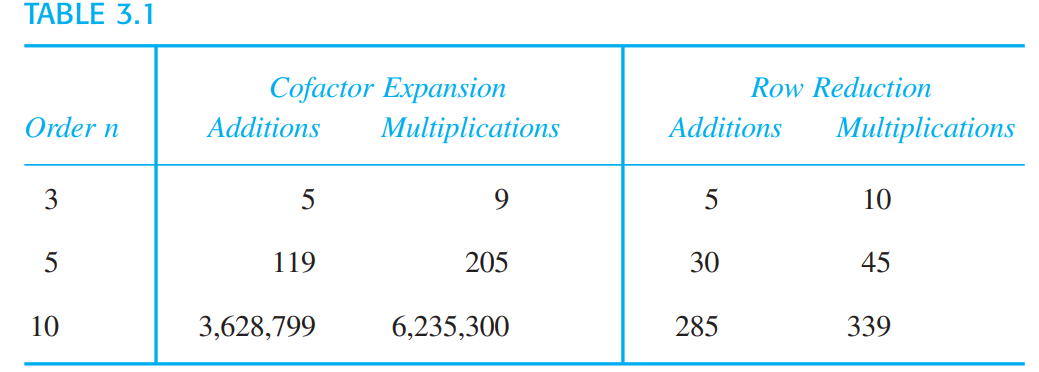
\includegraphics[width = 12cm]{images/numoperationfordet.png}
        \end{center}
        For this reasons, most computer and calculator algorithm use the method involving elementary row operations.

        In fact, the number of operations for the cofactor expansion of an $n \x n$ matrix grows like $n!$. Because 
        $30! \approx 2.65 \x 10^{32}$, even a relatively small $30 \x 30$ matrix would require more than $10^{32}$ operations.

        \subsubsection*{\textcolor{blue}{Techniques}}

        Create a row or column having all zeros in all but one position - then using cofactor expansion to reduce
        the order of the matrix by $1$.
        \begin{equation*}
          A =  \left|\begin{tblr}{
            colspec = {cccc},
            cell{1}{1} = {blue9},
            cell{2}{1} = {blue9},
            cell{3}{1,2,3} = {blue9}}
            -3 & 5 & -4 \\
            2 & -4 & 3 \\
            -3 & 0 & 0
             \end{tblr}\right|  = (-3)(-1)^{4} \begin{vmatrix}
            5 & -4 \\-4 & 3
             \end{vmatrix} = 3
        \end{equation*} 


    \section{Properties of Determinants}

    \begin{tcolorbox}[hbox]
    \B{Determinant of a Product.}
        \centering
        $|A_1A_2\cdots A_k| = |A_1||A_2|\cdots |A_k|$
    \end{tcolorbox}

    \B{\textit{Proof.}}
    \quad If $E$ is an elementary matrix, 
    \begin{enumerate}
        \item Interchanging 2 rows of $I$ : $|E| = -1$
        \item Multiplying a row of I by $c$ : $|E| = c$
        \item Adding a multiple of 1 row of $I$ to another row of $I$ : $|E| = 1$ 
    \end{enumerate}
        It follows that, $|EB| = |E|.|B|$. This can be generalized to conclude that
        \[ |E_k \dots E_2 E_1 B| = |E_k| \cdots |E_2| |E_1|.|B| \]
    Now consider the matrix $AB$. If $A$ is \textbf{nonsingular}, then it can be written as $E_k \dots E_2E_1$ and we can write
    \[ |AB| = |E_k| \cdots |E_2| |E_1| |B| = |E_k \cdots E_2 E_1| |B| = |A||B|\]
    If $A$ is \B{singular}, then it is row-equivalent to a matrix with an entire row of zeros. Moreover, we
    can conclude that $AB$ is also \B{singular}.

    \begin{tcolorbox}[hbox]
    \B{Determinant of a Scalar Multiple of a Matrix.} $|cA| = c^n|A|$
    \end{tcolorbox}

    \B{\textit{Proof.}} Factor the scalar $c$ out of each rows of $|cA|$, proof complete.

    \subsection{Determinants and the Inverse of a Matrix}

    \begin{tcolorbox}[hbox]
        \B{Determinant of an invertible matrix.} $det(A) \neq 0$
    \end{tcolorbox}
    
    \B{\textit{Proof.}} 

    1. Assume $A$ is invertible $\Leftrightarrow AA^{-1} = I$.
    
    $\Leftrightarrow |A| |A^{-1}| = |I| = 1$. Then neither $|A|$ nor $|A^{-1}|$ is $0$.
    
    2. Assume $|A| \ne 0$. 

    Using Gauss-Jordan elimination, find a matrix $B$ in row-echelon form that is row-equivalent
    to $A$. This implies, $B = I_n$ or $B$ has at least 1 row that consists entirely of 0 - $|B| = 0$ which leads to $|A| = 0$.
    So $B$ must be $I_n$.

    $A$ is, therefore, row-equivalent to the identity matrix - in other words, it is \B{invertible}.

    \begin{tcolorbox}[hbox, colback = {blue9}]
        \B{Determinant of an Inverse Matrix.}
        $|A^{-1}| = \frac{1}{|A|}$
    \end{tcolorbox}
    \B{\textit{Proof.}} Since $|A|.|A^{-1}| = 1$, proof complete.

    \subsection{Equivalent Conditions for a Nonsingular Matrix}

    \begin{tcolorbox}[colback = {blue9}]
        If $A$ is an $n \x n$ matrix, the following statements are equivalent.
        \begin{enumerate}
            \item $A$ is \B{invertible}.
            \item $A$\B{x} = \B{b} has a \B{unique solution} for EVERY $n \x 1$ column matrix \B{b}
            \item $A$\B{x} = $P$ has only the trivial solution.
            \item $A$ is row-equivalent to $I_n$.
            \item $A$ can be written as product of elementary matrices.
            \item $det(A) \ne 0$
        \end{enumerate}
    \end{tcolorbox}

    \B{REMARK. } $A$ can have a determinant of zaro if $A$ is row-equivalent to a matrix that has at least one row
    consisting entirely of zeros. (Properties $4$ and $6$)

    \subsection{Determinants and the Transpose of a Matrix}
    \tcl
        \B{Determinant of a Transpose. } $det(A) = det(A^T)$
    \etcl

    \section{Introduction to Eigenvalues}
    This is one of the most important topics of linear algebra - \B{eigenvalues}. One applicaion of eigenvalues
    involves the study of population growth. 

    \textbf{Example.} Suppose that half of a population of rabbits raised in a laboratory
    survive their first year. Of those, half survive their second year. Their maximum life span is
    3 years. Furthermore, during the first year the rabbits produce no offspring, whereas the
    average number of offspring is 6 during the second year and 8 during the third year. If there
    are 24 rabbits in each age class now, what will the distribution be in 1 year? In 20 years?

    \tcl
    \B{Eigenvalue problem.} If $A$ is an $n \x n$ matrix, do there exist $n \x 1$ nonzero matrices $x$ such that $A$\B{x} is a scalar
    multiple of \B{x}?
    \begin{itemize}
        \item \B{eigenvalue} of $A$: $\lambda$ \textit{(the scalar)}
        \item \B{eigenvector} of $A$: \B{x} \textit{(corresponding to $\lambda$)}
    \end{itemize}
    The fundamental equation for the eigenvalue problem is
    \[ Ax = \lambda x\]
    \etcl

    \B{Example 1.} Let $A = \begin{bmatrix}
        1 & 4 \\
        2 & 3
    \end{bmatrix}, \quad x_1 = \begin{bmatrix}
        1 \\ 1
    \end{bmatrix}, \quad x_2 = \begin{bmatrix}
        2 \\ -1
    \end{bmatrix}$\\
    That is, $\lambda_1 = 5$ is an \B{eigenvalue} of $A$ corresponding to $x_1$, and $\lambda_2 = -1$ is an \B{eigenvalue} of $A$
    corresponding to $x_2$.

    \B{Notice.} If $x$ is an eigenvector corresponding to $\lambda$, then so is \B{any nonzero multiple of x}.
    
    \subsection{Finding Eigenvalues and Eigenvectors}
    \tcl
    Provided with an $n \x n$ matrix, how to find the \B{eigenvalues} and the corresponding \B{eigenvector}?
    The key is to write the equation $A$\B{x} = $\lambda$\B{x} in the equivalent form
    \[ (\lambda I - A)\B{x} = 0 \text{\textit{(characteristic equation)}}\]
    \etcl
    This \B{homogeneous} system of equations has nonzero solutions if and only if the coefficient matrix 
    $(\lambda I - A)$ is \B{singular} - that is,\[det(\lambda I - A) = 0\] That equation is called the \B{characteristic 
    equation} of $A$ - and is a polynomial equation of degree $n$ in the variable $\lambda$. Once we have found the
    \B{eigenvalues} of $A$, you can use Gaussion elimination to find the corresponding eigenvectors.

    \B{Example 2.} Find eigenvalues and corresponding eigenvectors of the matrix $A = \begin{bmatrix}
        1 & 4\\
        2 & 3
    \end{bmatrix}$

    \textit{SOLUTION. } The characteristic equation of $A$ is 
    \begin{equation*}
        \begin{split}
            |\lambda I - A| & = \left| \begin{bmatrix}
                \lambda & 0 \\
                0 & \lambda
            \end{bmatrix} - \begin{bmatrix}
                1 & 4 \\
                2 & 3
            \end{bmatrix}\right| \\
                            & = \begin{vmatrix}
                                \lambda - 1 & -4 \\
                                -2 & \lambda - 3
                            \end{vmatrix} \\
                            & = \lambda ^2 - 4\lambda - 5 \\
                            & = (\lambda - 5)(\lambda + 1) = 0
        \end{split}
    \end{equation*}
    For $\lambda_1 = 5$, the coefficient matrix is $5I - A = \begin{bmatrix}
        4 & -4 \\
        -2 & 2
    \end{bmatrix}$, which row reduced to $ \begin{bmatrix}
        1 & -1 \\
        0 & 0
    \end{bmatrix}$.

    The solutions of the homogeneous system having this coefficient matrix are all of the form $ \begin{bmatrix}
        t \\ t
    \end{bmatrix}$.
    So, the \B{eigenvectors} corresponding to the \B{eigenvalue} $\lambda_1 = 5$ are the nonzero scalar multiples of 
    $ \begin{bmatrix}
        1 \\ 1
    \end{bmatrix}$.

    And the eigenvectors corresponding to the eigenvalue $\lambda_2 = -1$ are the nonzero scalar multiples of
    $ \begin{bmatrix}
        2 \\ -1
    \end{bmatrix}$.
    
    \B{Example 3.} Find the eigenvalues and corresponding eigenvectors of the matrix
    \[ A = \begin{bmatrix}
        1 & 2 & -2\\
        1 & 2 & 1\\
        -1 & -1 & 0
    \end{bmatrix}\]

    \textit{SOLUTION. }The characteristic equation of $A$ is
    \begin{equation*}
        \begin{split}
            |\lambda I - A|  & = \left| \begin{bmatrix}
            \lambda - 1 & -2 & 2\\
            -1 & \lambda - 2 & -1\\
            1 & 1 & \lambda
        \end{bmatrix} \right| \\
         & = (\lambda - 1) \begin{vmatrix}
             \lambda - 2 & -1\\
             1 & \lambda
         \end{vmatrix} - (-2) \begin{vmatrix}
             -1 & -1 \\
             1 & \lambda
         \end{vmatrix} +
         2 \begin{vmatrix}
             -1 & \lambda - 2 \\
             1 & 1
         \end{vmatrix} \\
         & = \lambda^3 - 3\lambda^2 - \lambda + 3 \\
         & = (\lambda^2 - 1)(\lambda - 3) = 0
        \end{split}
    \end{equation*}
    For $\lambda_1 = 1$, the coefficient matrix is
    \[ I - A = \begin{bmatrix}
        0 & -2 & 2\\
        -1 & -1 & -1\\
        1 & 1 & 1
    \end{bmatrix}\]
    which row reduces to $ \begin{bmatrix}
        1 & 0 & 2 \\
        0 & 1 & -1\\
        0 & 0 & 0
    \end{bmatrix}$.
    
    The solutions of the homogeneous system having this coefficient matrix are all of the form $ \begin{bmatrix}
        -2t \\ t \\ t
    \end{bmatrix}$.
    where $t$ is a real number. \\So, the eigenvectors corresponding to the eigenvalue $\lambda_1 = 1$ are the nonzero scalar
    multiples of $ \begin{bmatrix}
        -2 \\ 1 \\ 1
    \end{bmatrix}$.
    
    Similarly, solve for $\lambda_2 = -1$ and $\lambda_3 = 3$.

    In \B{Chapter 7}, we will study eigenvalues and their applicaions in more detail.

    \section{Applications of Determinants}

    \subsection{The Adjoint of a Matrix}

    If $A$ is a square matrix, then the \B{matrix of cofactors} of $A$ has the form
    \[ \begin{bmatrix}
        C_{11} & C_{12} & \cdots & C_{1n} \\
        C_{21} & C_{22 } & \cdots & C_{21}\\
        \vdots & \vdots & & \vdots \\
        C_{n1} & C_{n2} & \cdots & C_{nn}
    \end{bmatrix} \]
    The transpose of this matrix is called the \B{adjoint} of $A$ and is denoted by
    \[ \text{adj}(A) = \begin{bmatrix}
        C_{11} & C_{21}  & \cdots & C_{n1} \\
        C_{12} & C_{22} &  \cdots & C_{n2} \\
        \vdots & \vdots & & \vdots \\
        C_{1n} & C_{2n}  & \cdots & C_{nn}
    \end{bmatrix} \]
        
    \begin{tcolorbox}[colback = {blue9}]
        \B{The Inverse of a Matrix Given by Its Adjoint.}
        If $A$ is an $n \x n$ invertible matrix, then
        \[ A^{-1} = \frac{1}{det(A)} \text{adj}(A) \]
    \end{tcolorbox}
    \textbf{\textit{Proof.}} Consider the product
    \begin{equation*} 
        \begin{split} 
            A[\text{adj}(A)] & = \begin{bmatrix}
        a_{11} & a_{12} & \cdots & a_{1n    } \\
        a_{21} & a_{22} & \cdots & a_{2n} \\
        \vdots & \vdots & & \vdots \\
        a_{n1} & a_{n2} & \cdots & a_{nn}
    \end{bmatrix} \begin{bmatrix}
        C_{11} & C_{21} & \cdots & C_{n1} \\
        C_{12} & C_{22} & \cdots & C_{n2} \\
        \vdots & \vdots & &  \vdots \\
        C_{1n}  & C_{2n} & \cdots & C_{nn}
    \end{bmatrix} \\
        & = det(A)I
            \end{split} 
        \end{equation*}
    \B{REMARK. } Using Gauss-Jordan elimination is much better. This theorem just provides a concise formula.

    \subsection{Cramer's Rule}
    \tcl
    If a system of $n$ linear equatios in $n$ variables has a coefficient matrix with a nonzero determinant
    $|A|$, then the solution of the system is given by
    \[ x_1 = \frac{det(A_1)}{det(A)}, \quad x_2 = \frac{det(A_2)}{det(A)}, \quad \dots, \quad x_n = \frac{det(A_n)}{det(A)}\]
    where the $i$th column of $A_i$ is the column of constants in the system of equations.
    \etcl
    \B{\textit{Proof.}} Let the system be represented by $AX = B$. Since $|A| \ne 0$, you can write
    \[ X = A^{-1}B = \frac{1}{|A|} adj(A)B = \begin{bmatrix}
        x_1 \\ x_2 \\ \vdots \\ x_n
    \end{bmatrix} \]
    If the entries of $B$ are $b_1, b_2, \dots, b_n$ then
    \[ x_i = \frac{1}{|A|} \sum_{j = 1}^n b_jC_{ji} = \frac{|A_i|}{|A|}\]

    \subsection{Area, Volume, and Equation of Lines and Planes}






\end{document}
